\documentclass[tikz,margin=10pt]{standalone}
    \usetikzlibrary{arrows.meta,chains,%
                    decorations.pathreplacing}

\begin{document}
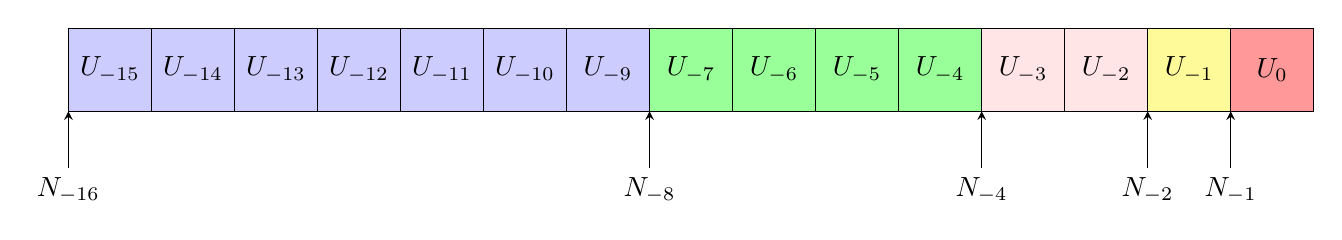
\begin{tikzpicture}[
  font=\ttfamily,
%  -{Stealth[length = 2.5pt]},
  start chain = going right,
     node distance = 0pt,
MyStyle/.style={draw, minimum width=3em, minimum height=3em,
                outer sep=0pt, on chain, fill=blue!20},
  ]
\node [MyStyle] (1) {$U_{-15}$};
\node [MyStyle] (2) {$U_{-14}$};
\node [MyStyle] (3) {$U_{-13}$};
\node [MyStyle] (4) {$U_{-12}$};
\node [MyStyle] (5) {$U_{-11}$};
\node [MyStyle] (6) {$U_{-10}$};
\node [MyStyle] (7) {$U_{-9}$};
\node [MyStyle, fill=green!40] (9) {$U_{-7}$};
\node [MyStyle, fill=green!40] (10) {$U_{-6}$};
\node [MyStyle, fill=green!40] (11) {$U_{-5}$};
\node [MyStyle, fill=green!40] (12) {$U_{-4}$};
\node [MyStyle, fill=pink!40] (13) {$U_{-3}$};
\node [MyStyle, fill=pink!40] (14) {$U_{-2}$};
\node [MyStyle, fill=yellow!40] (15) {$U_{-1}$};
\node [MyStyle, fill=red!40] (16) {$U_{0}$};

\node [yshift=-1cm] at (15.south east) (n1) {$N_{-1}$};
\draw [-stealth] (n1) -- (15.south east);


\node [yshift=-1cm] at (14.south east) (n2) {$N_{-2}$};
\draw [-stealth] (n2) -- (14.south east);

\node [yshift=-1cm] at (12.south east) (n3) {$N_{-4}$};
\draw [-stealth] (n3) -- (12.south east);

\node [yshift=-1cm] at (7.south east) (n4) {$N_{-8}$};
\draw [-stealth] (n4) -- (7.south east);


\node [yshift=-1cm] at (1.south west) (n5) {$N_{-16}$};
\draw [-stealth] (n5) -- (1.south west);
\end{tikzpicture}
  \end{document}